\section{Second Section}
This is another section.

\subsection{First Subsection}
This is a subsection.

\subsubsection{First Subsubsection}
\label{sec:subsubectionname}
Lorem ipsum dolor sit amet, consetetur sadipscing elitr, sed diam nonumy eirmod tempor invidunt ut labore et dolore magna aliquyam erat, sed diam voluptua. At vero eos et accusam et justo duo dolores et ea rebum.

Stet clita kasd gubergren, no sea takimata sanctus est Lorem ipsum dolor sit amet. Lorem ipsum dolor sit amet, consetetur sadipscing elitr, sed diam nonumy eirmod tempor invidunt ut labore et dolore magna aliquyam erat, sed diam voluptua. At vero eos et accusam et justo duo dolores et ea rebum. Stet clita kasd gubergren, no sea takimata sanctus est Lorem ipsum dolor sit amet.

Lorem ipsum dolor sit amet, consetetur sadipscing elitr, sed diam nonumy eirmod tempor invidunt ut labore et dolore magna aliquyam erat, sed diam voluptua. At vero eos et accusam et justo duo dolores et ea rebum.

\begin{figure}
\centering
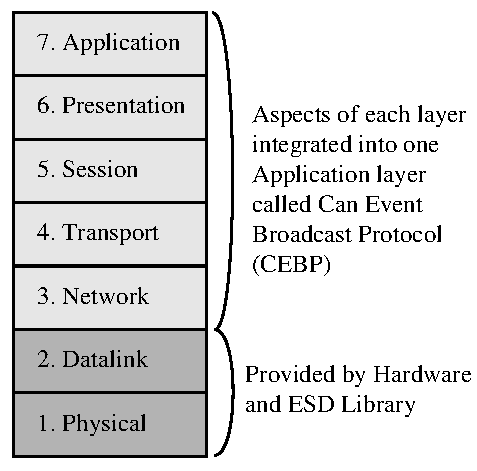
\includegraphics[width=7cm]{pictures/OSI.pdf} % You can also use JPG, PNG etc.
\caption{Open System Interconnection}
\label{fig:OSI}
\end{figure}

Figures \ref{fig:OSI} can be referenced with the command \verb|\ref{fig:mylabel}|. A table could look like Table~\ref{tab:systemcomparison}.

\begin{table*}[htbp]
    \centering
    \begin{tabular}{lccc} \toprule
        \textbf{Item}      & \textbf{Multiprocessor} & \textbf{Multicomputer}  & \textbf{Distributed System} \\\midrule
        node configuration & CPU                     & CPU, RAM, net interface & complete computer           \\\midrule
        node peripherals   & all shared              & shared exc., maybe disk & full set per node           \\\midrule
        location           & same rack               & same room               & possibly worldwide          \\\midrule
        internode comm.    & shared RAM              & dedicated interconnect  & traditional network         \\\midrule
        operating system   & one, shared             & multiple, same          & possibly all different      \\\midrule
        file systems       & one, shared             & one, shared             & each node has own           \\\midrule
        administration     & one organization        & one organization        & many organizations          \\\bottomrule
    \end{tabular}
    \caption{Comparison (2-column table) with \texttt{table*} instead of \texttt{table}}
    \label{tab:systemcomparison} % Die Reihenfolge ist wichtig: Erst \caption, dann \label!
\end{table*}

\noindent An \texttt{enumerate} environment:
\begin{enumerate}
\item Point
\item Point
\end{enumerate} 

\noindent An \texttt{itemize} enviroment:
\begin{itemize}
\item Bullet point
\item Bullet point
\end{itemize}

The \verb|\enquote| command is helpful for correct \enquote{portable} quotation marks. Just put your quote in the command: \verb|\enquote{This is a quote.}| gets \enquote{This is a quote.}

\subsubsection{Citations}
You have to cite literature in your seminar thesis. Use the command \verb|\cite| for citations. For citing the publication \texttt{ROFES} from \texttt{literature.bib}, use the command \verb|\cite{ROFES}| \cite{ROFES}. You might also find the command \verb|\textcite| useful which additionally shows the authors in the text: \textcite{ROFES}

\subsubsection{Units}
Use \verb|\unit| and \verb|\unitfrac| commands for typesetting units, e.g. \unitfrac[100]{MBit}{s}, \unit[10]{MB}, \unit[1]{s}.

